\documentclass{standalone}
\usepackage{pgfplots}
\pgfplotsset{compat=1.18}

\begin{document}

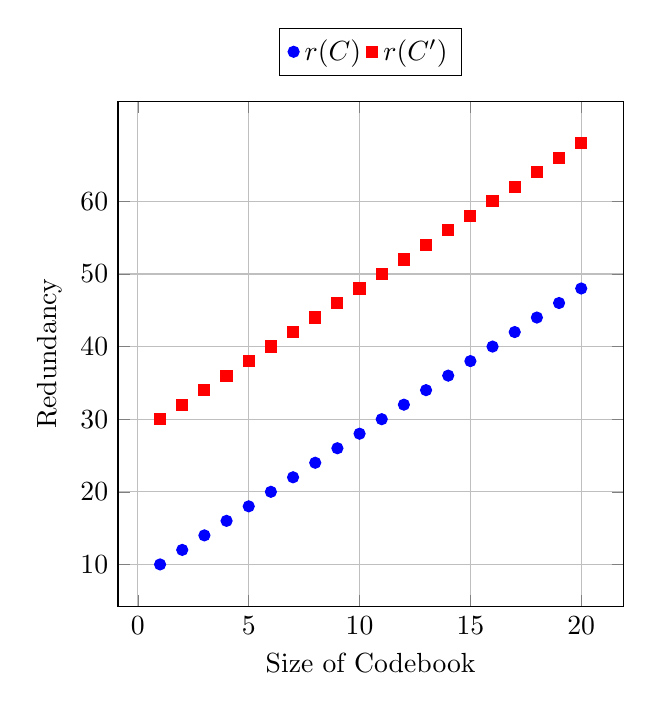
\begin{tikzpicture}
    \begin{axis}[
        width=8cm,
        height=8cm,
        xlabel={Size of Codebook},
        ylabel={Redundancy},
        legend style={at={(0.5,1.05)},anchor=south,legend columns=-1},
        xtick={0,5,10,15,20},
        ytick={0,10,20,30,40,50,60},
        grid=major,
        legend cell align={left}
    ]
    \addplot[
        color=blue,
        mark=*,
        only marks
    ]
    coordinates {
        (1,10)(2,12)(3,14)(4,16)(5,18)
        (6,20)(7,22)(8,24)(9,26)(10,28)
        (11,30)(12,32)(13,34)(14,36)(15,38)
        (16,40)(17,42)(18,44)(19,46)(20,48)
    };
    \addplot[
        color=red,
        mark=square*,
        only marks
    ]
    coordinates {
        (1,30)(2,32)(3,34)(4,36)(5,38)
        (6,40)(7,42)(8,44)(9,46)(10,48)
        (11,50)(12,52)(13,54)(14,56)(15,58)
        (16,60)(17,62)(18,64)(19,66)(20,68)
    };
    \legend{$r(C)$,$r(C')$}
    \end{axis}
\end{tikzpicture}

\end{document}